\documentclass[handout]{beamer}

\usetheme{Warsaw}

\usepackage[brazil]{babel}
\usepackage[latin1]{inputenc}
\usepackage{times}
\usepackage[T1]{fontenc}
\usepackage{epsfig}
\usepackage{listings}
\usepackage{amsfonts}
\usepackage{multirow}
\usepackage{tikz}
\usepackage{textpos}
\usepackage{framed, multicol}
\usepackage{wrapfig}
\usepackage{array}
\usepackage{booktabs}
\usepackage{verbatim}
\usepackage{tikz}
\usepackage{tikz-uml}


%\usepackage{dcolumn}
%\newcolumntype{.}{D{.}{.}{-1}}
%\newcolumntype{d}[1]{D{.}{.}{#1}}
%\usetheme{Berkeley}

\newcommand{\be}{\begin{enumerate}[<+->]}
\newcommand{\ee}{\end{enumerate}}

\newcommand{\bq}{\begin{quote}}
\newcommand{\eq}{\end{quote}}

\newcommand{\bd}{\begin{description}[<+->]}
\newcommand{\ed}{\end{description}}

\newcommand{\bi}{\begin{itemize}[<+->]}
\newcommand{\ei}{\end{itemize}}

\newcommand{\bbl}{\begin{block}{Exemplo: Tipos primitivos do Pascal}
        \scriptsize
        \centering
        }
\newcommand{\ebl}{\end{block}}




%%%%%%%%%%%%%%%%%%%%%%%%%%%%%%%%%%%%%%%%%%%%%%%%%%%%%%%%%%%%%%%%
% Configuração do Tiks
%%%%%%%%%%%%%%%%%%%%%%%%%%%%%%%%%%%%%%%%%%%%%%%%%%%%%%%%%%%%%%%%
\usetikzlibrary{arrows}

\tikzstyle{bloco}=[draw, minimum size=2em] %fill=blue!20,
\tikzstyle{linha} = [pin edge={to-,thin,black}]



\title[Programa��o Modular]
{%
    Java I/O%
}
\author[Prof. Pedro Pongelupe]
{
    Prof.~Pedro~Pongelupe
}
\institute[DCC / PUC Minas]
{
\includegraphics[width=4cm]{puc_engesoft_logo.png} \\
  \textsc{Pontif�cia Universidade Cat�lica de Minas Gerais}\\
    Curso de Engenharia de Software
}

\date[]{}

\lstset{language=Java,
   basicstyle=\scriptsize,
   commentstyle=\color{red},
   showstringspaces=false,
   numbers=none,
   numberstyle=\tiny}

\begin{document}


\selectlanguage{brazil}

\begin{frame}
   \titlepage
\end{frame}

%\addtobeamertemplate{frametitle}{}{%
%    \begin{tikzpicture}[remember picture,overlay]
%    \node[anchor=north east,yshift=2pt] at (current page.north east) {
\epsfig{file=puclogo_small_bw,width=1.2cm}};
%    \end{tikzpicture}}


%\addtobeamertemplate{frametitle}{}{%
    %\begin{tikzpicture}[node distance=0cm, remember picture, overlay, every node/.style={inner sep=0,outer sep=0, node distance=0cm, baseline=0cm}]
    %\node[anchor=north east] at (current page.north east) {
\epsfig{file=puclogo_small_bw,width=1cm}};
    %\end{tikzpicture}}


%\logo{
\includegraphics[height=0.8cm]{puclogo_small_bw.pdf}\vspace{220pt}}


\begin{frame}
   \frametitle{Sum�rio}
   \tableofcontents[pausesections]
\end{frame}

%\AtBeginSection[] % Do nothing for \section*
%{
%\begin{frame}<beamer>
%\frametitle{Outline}
%\tableofcontents[currentsection]
%\end{frame}}

% duas   linhas 1.48cm
% tres   linhas 1.75cm
% quatro linhas 2.02cm
% cinco  linhas 2.26cm
\addtobeamertemplate{frametitle}{}{%
	\begin{textblock*}{10mm}(.8785\textwidth,-1.75cm)
		
\includegraphics[height=0.97cm]{puc_engesoft_logo.png}%
\includegraphics[height=1cm]{puclogo_small_bw.pdf}
	\end{textblock*}
}
%\addtobeamertemplate{frametitle}{}{%
%   \begin{textblock*}{10mm}(.9945\textwidth,-1.71cm)
%    
\includegraphics[height=1cm]{puclogo_small_bw.pdf}
%   \end{textblock*}
%}

\section{Java I/O Streams}

\subsection{Interfaces base}

\begin{frame}[fragile]{I/O Streams}

\begin{itemize}
\item Byte Streams -- classes abstratas:
\begin{itemize}
\item \lstinline|InputStream|
\item \lstinline|OutputStream|
\end{itemize}
\item Character Streams -- classes abstratas:
\begin{itemize}
\item \lstinline|Reader|
\item \lstinline|Writer|
\end{itemize}

\end{itemize}

\end{frame}

\subsection{Destinos}

\begin{frame}[fragile]{Destinos de leitura/escrita}

\begin{itemize}
\item Arquivo:
\begin{itemize}
\item \lstinline|FileInputStream, FileOutputStream|
\item \lstinline|FileReader, FileWriter|
\end{itemize}
\item Arranjos (vetores):
\begin{itemize}
\item \lstinline|ByteArrayInputStream, ByteArrayOutputStream|
\item \lstinline|CharArrayReader, CharArrayWriter|, ``\lstinline|StringReader, StringWriter|''
\end{itemize}
\item Pipes:
\begin{itemize}
\item \lstinline|PipedInputStream, PipedOutputStream|
\item \lstinline|PipedReader, PipedWriter|
\end{itemize}
\item Mem�ria: 
\begin{itemize}
\item \lstinline|BufferedInputStream, BufferedOutputStream|
\item \lstinline|BufferedReader, BufferedWriter|
\end{itemize}
\end{itemize}
\end{frame}

\section{Exemplo: Arquivo}


\begin{frame}[fragile]{Exibe arquivo}

\begin{lstlisting}
public static void main(String args[]) {
   int i;
   FileInputStream fin = null;
    try {
      fin = new FileInputStream(args[0]);
       do {
           i = fin.read();
           if (i != -1)      System.out.print((char) i);
       } while (i != -1);
   } catch (FileNotFoundException exc) {
       System.out.println("Arquivo " + args[0] + " n�o encontrado.");
   } catch (IOException exc) {
       System.out.println("Erro de entrada/sa�da");
   } finally {
           try {
           if (fin != null)  fin.close();
       } catch (IOException exc) {
           System.out.println("Erro ao fechar arquivo.");
       }
   }
}
\end{lstlisting}
\end{frame}

\subsection{Fechamento autom�tico}

\begin{frame}[fragile]{Fechamento autom�tico de arquivo}

\begin{lstlisting}
public static void main(String args[]) {
    int i;
    if (args.length != 1) {
        System.out.println("Usage: ShowFile filename");
        return;
    }
    try (FileInputStream fin = new FileInputStream(args[0])) {
        do {
            i = fin.read();
            if (i != -1)
                System.out.print((char) i);
        } while (i != -1);
    } catch (FileNotFoundException exc) {
        System.out.println("File Not Found.");
    } catch (IOException exc) {
        System.out.println("An I/O Error Occurred");
    }
}
\end{lstlisting}
\end{frame}


\subsection{Acesso aleat�rio}

\begin{frame}[fragile]{Arquivos com acesso aleat�rio}
\begin{lstlisting}
public static void main(String args[]) {
  double dados[] = { 42.5, 102.1, 123.45, 33.0, 111.1, 543.21 };
  double d;

  try (RandomAccessFile arq = 
          new RandomAccessFile("binario.dat", "rw")) {
    for (int i = 0; i < dados.length; i++) {
        arq.writeDouble(dados[i]);
    }
    arq.seek(8);
    d = arq.readDouble();
    System.out.println("2o valor: " + d);
    for (int i = 0; i < dados.length; i++) {
       arq.seek(8 * i);
       d = arq.readDouble();
       System.out.print(d + " ");
    }
  } catch (IOException e) {
    System.out.println("Erro de I/O: " + e);
  }
}
\end{lstlisting}
\end{frame}

\section{Data Access Object}

\subsection{DAO Factory Pattern}

%
\begin{frame}[fragile]{Data Access Object Pattern}
\begin{itemize}
  \item DAO Pattern: usado para separar as APIs de acesso a dados das classes de neg�cios.
\end{itemize}

\begin{center}
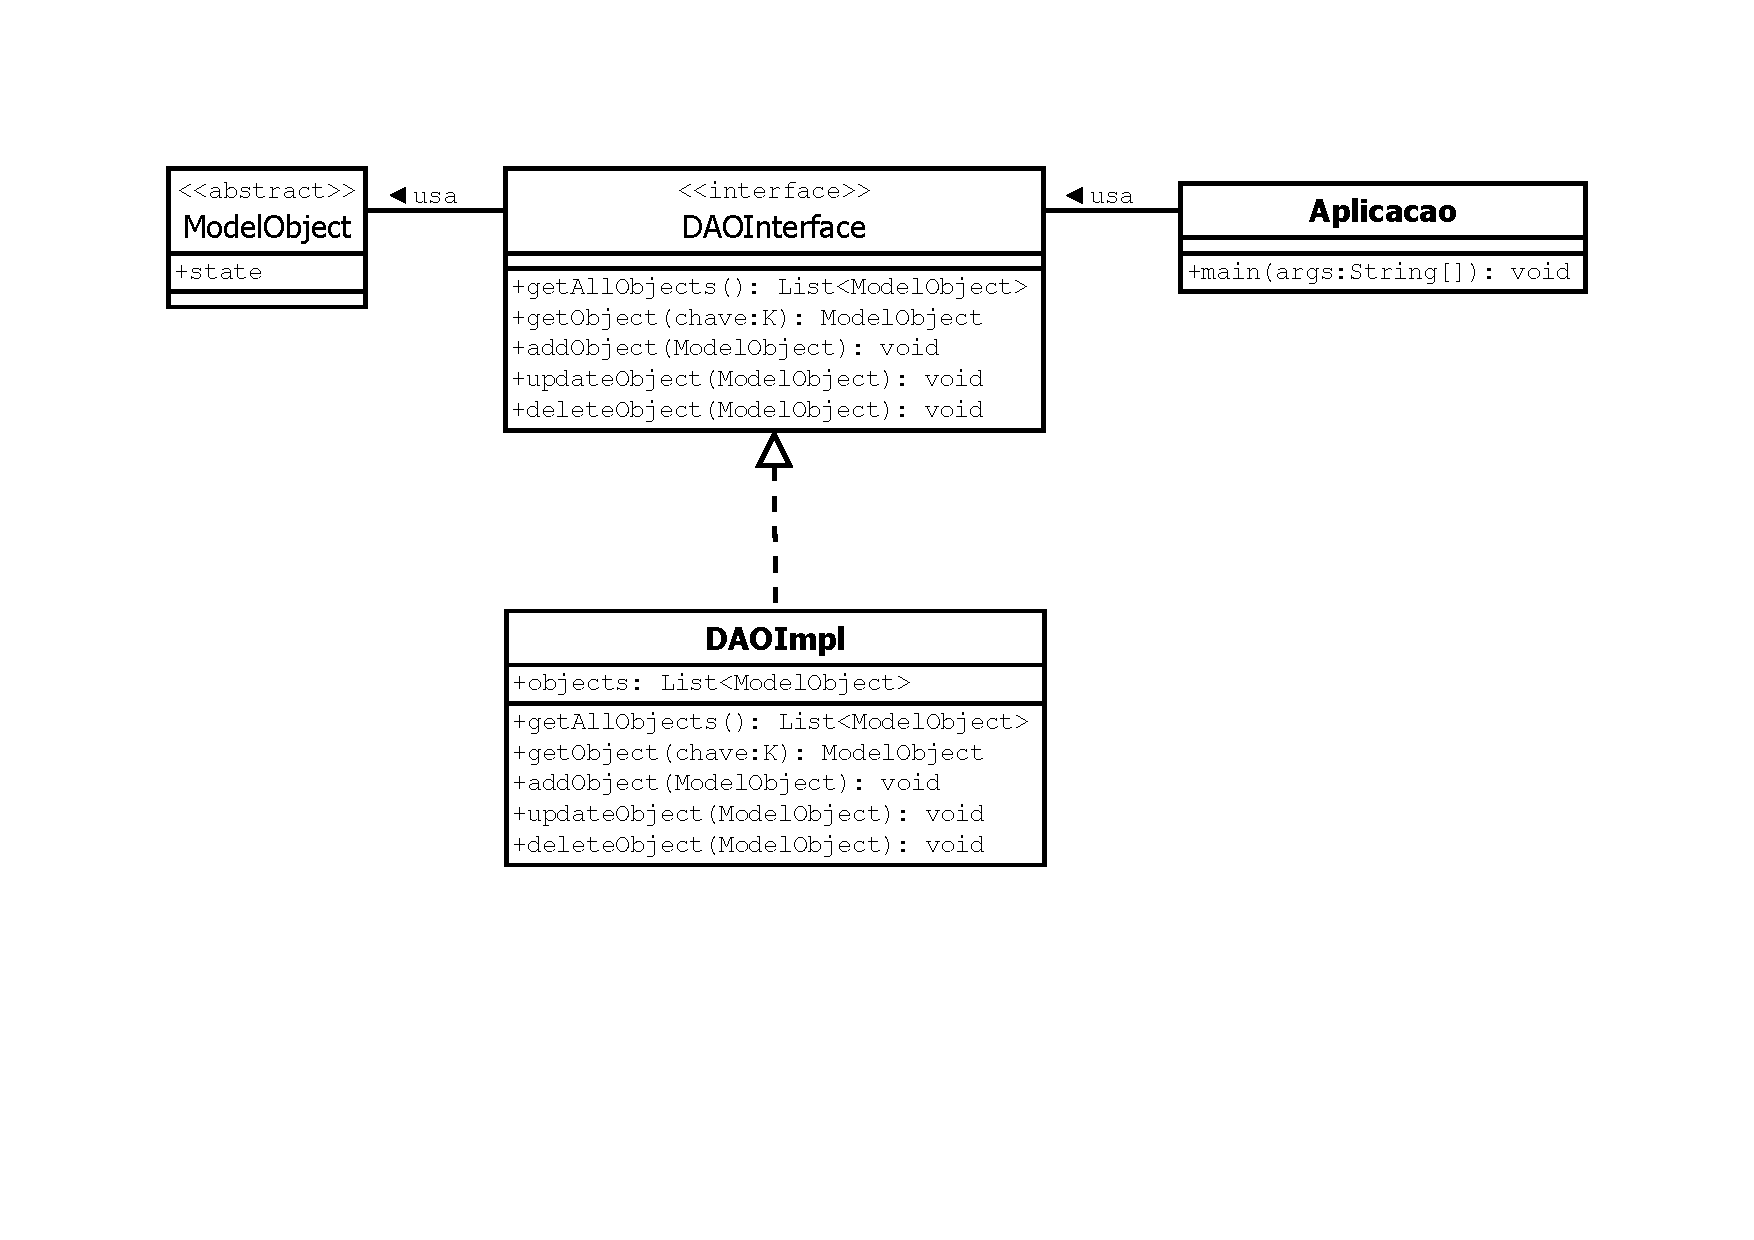
\includegraphics[width=.9\textwidth]{daopattern.pdf}
\end{center}
\end{frame}


\subsection{Tipagem}

\begin{frame}[fragile]{Leitura/Escrita Tipada}
    
    \begin{itemize}
        \item Tipos primitivos: \lstinline|DataInputStream, DataOutputStream|
        \item Objetos de classe: \lstinline|ObjectInputStream, ObjectOutputStream|
        \begin{itemize}
            \item Objeto deve ser serializ�vel:  \lstinline|implements Serializable|
        \end{itemize}
    \end{itemize}
\end{frame}


\begin{frame}[fragile]{Classes Serializ�veis}
    
    \begin{itemize}
    \item \lstinline|Serializable| � chamada \textit{markup interface}, porque n�o possui m�todos.
    \item Java ir� converter o objeto para bin�rio.
\end{itemize}
    
\begin{lstlisting}
  abstract class Produto implements Serializable
  
  public class BemDuravel extends Produto implements Serializable
  
  public class BemDeConsumo extends Produto implements Serializable
  
\end{lstlisting}
\end{frame}

\begin{frame}[fragile]{DAO bin�rio polim�rfico}
    
    \begin{itemize}
        \item \lstinline|Serializable| � chamada \textit{markup interface}, porque n�o possui m�todos.
        \item O Java ir� converter o objeto para bin�rio.
    \end{itemize}
    
    \begin{lstlisting}
public class ProdutoDAO {
  private ObjectOutputStream outputFile;
  ...
   
  public void add(Produto produto) throws IOException {

        outputFile.writeObject(produto);
   }
}

ProdutoDAO bemDeConsumoDAO = new ProdutoDAO("bemdeconsumo.bin");

bemDeConsumoDAO.add(new BemDeConsumo("Leite",    4.00F, 120, 
           LocalDateTime.now(), LocalDate.now().plusMonths(6)));


    \end{lstlisting}
\end{frame}


\begin{frame}[fragile]{Obrigado!!}
        Muito obrigado pela aten��o! Alguma d�vida? Bora praticar!!!
        \begin{block}{  }
                "\textit{O mundo � formado n�o apenas pelo que j� existe, mas pelo que pode efetivamente existir."}
        \end{block}
\end{frame}

\end{document}

